\documentclass{article}
\usepackage[paperwidth=1000pt, paperheight=800pt, margin=10pt]{geometry}
\usepackage{amsmath}
\usepackage{tikz}
\usetikzlibrary{matrix,positioning,decorations.pathreplacing}

\begin{document}
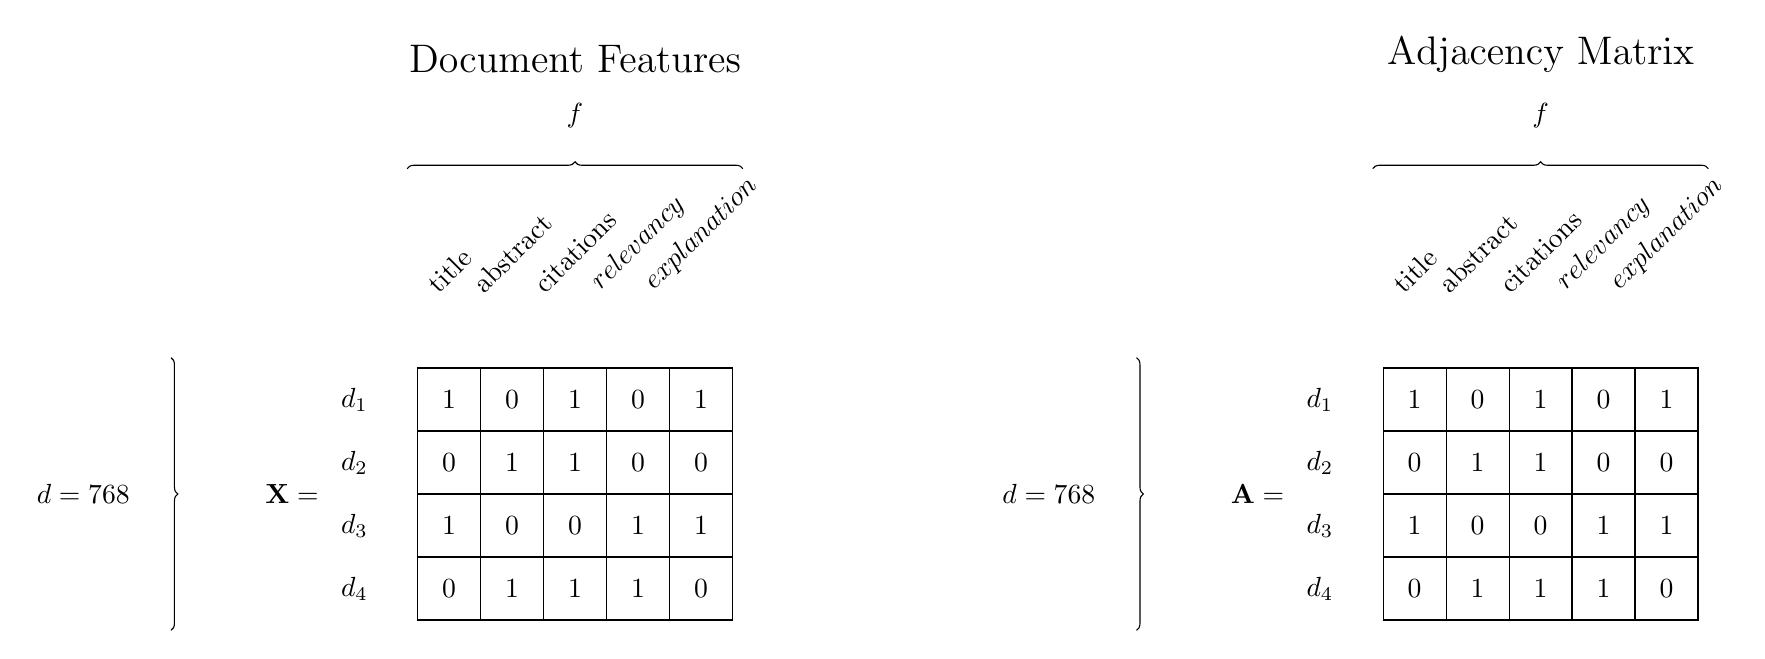
\begin{tikzpicture}[scale=3,
    node_matrix/.style={
        matrix of math nodes,
        nodes={draw, minimum size=8mm},
        nodes in empty cells,
        row sep=-\pgflinewidth,
        column sep=-\pgflinewidth,
    }
]

% Document Features Matrix
\matrix (X) [node_matrix] {
    1 & 0 & 1 & 0 & 1 \\
    0 & 1 & 1 & 0 & 0 \\
    1 & 0 & 0 & 1 & 1 \\
    0 & 1 & 1 & 1 & 0 \\
};

% Matrix Labels
\node[left=1cm of X] {$\mathbf{X} = $};
\node[above=3.5cm of X] {\Large Document Features};

% Row Labels
\foreach \i/\label in {1/d_1, 2/d_2, 3/d_3, 4/d_4} {
    \node[left=0.5cm] at (X-\i-1.west) {$\label$};
}

% Column Labels with mathematical notation
\foreach \i/\label in {1/\mathrm{title}, 2/\mathrm{abstract}, 3/\mathrm{citations}, 4/relevancy, 5/explanation} {
    \node[above=0.8cm] at (X-1-\i.north) {\rotatebox{45}{$\label$}};
}

% Adjacency Matrix
\matrix (A) [node_matrix, right=8cm of X] {
    1 & 0 & 1 & 0 & 1 \\
    0 & 1 & 1 & 0 & 0 \\
    1 & 0 & 0 & 1 & 1 \\
    0 & 1 & 1 & 1 & 0 \\
};

% Matrix Labels
\node[left=1cm of A] {$\mathbf{A} = $};
\node[above=3.5cm of A] {\Large Adjacency Matrix};

% Row Labels
\foreach \i/\label in {1/d_1, 2/d_2, 3/d_3, 4/d_4} {
    \node[left=0.5cm] at (A-\i-1.west) {$\label$};
}

\foreach \i/\label in {1/\mathrm{title}, 2/\mathrm{abstract}, 3/\mathrm{citations}, 4/relevancy, 5/explanation} {
    \node[above=0.8cm] at (A-1-\i.north) {\rotatebox{45}{$\label$}};
}


% Add braces to show matrix dimensions
\draw[decorate, decoration={brace, mirror}] 
    ([xshift=-1cm]X.south west) -- ([xshift=-1cm]X.north west)
    node[midway, left=0.4cm] {$d = 768$};
\draw[decorate, decoration={brace}]
    ([yshift=0.8cm]X.north west) -- ([yshift=0.8cm]X.north east)
    node[midway, above=0.4cm] {$f$};

\draw[decorate, decoration={brace, mirror}]
    ([xshift=-1cm]A.south west) -- ([xshift=-1cm]A.north west)
    node[midway, left=0.4cm] {$d = 768$};
\draw[decorate, decoration={brace}]
    ([yshift=0.8cm]A.north west) -- ([yshift=0.8cm]A.north east)
    node[midway, above=0.4cm] {$f$};

\end{tikzpicture}

\end{document}